\documentclass[a4paper,12pt,twoside]{article}
\usepackage[spanish]{babel}
\usepackage[utf8]{inputenc}
\usepackage{graphicx} %para insertar graficos/imagenes
\usepackage{amsmath} %para escribir matrices
\usepackage{amssymb}
\usepackage{amsfonts} %para poner \mathbb
\usepackage{float} %me deja usar la H de 'here' en los graficos para ponerlos donde yo quiera
\usepackage{anysize} %me permite definir los margenes como quiera
\usepackage{multirow} %para tablas con multicolumna
\usepackage{fancyhdr} % activamos el paquete
\usepackage{dcolumn}
\usepackage{multirow}
\usepackage{caption, subcaption}
\captionsetup[table]{textfont=it,position=top}
\usepackage{booktabs}

\usepackage[output-decimal-marker={,}]{siunitx} %Para las unidades. Tengo la versión 2

\usepackage[font=footnotesize, labelfont=bf, margin=2.2cm]{caption}

\usepackage{fixme}
\fxsetup{
    status=draft,
    author=,
    layout=inline, % also try footnote or pdfnote
}

\usepackage[T1]{fontenc}

\newcommand{\grad}{$^\circ$}
\newcommand{\codigoMateria}{66.44}
\newcommand{\nombreMateria}{Instrumentos Electrónicos}
\newcommand{\nroTP}{1}
\newcommand{\descripcionTP}{Trabajo práctico}
\newcommand{\tituloTP}{Trabajo}
\newcommand{\facultad}{Facultad de Ingeniería}
\newcommand{\universidad}{Universidad de Buenos Aires}
\newcommand{\docentes}{Enrique Zothner}

\pagestyle{fancy} % seleccionamos un estilo
\fancyhead{}
\fancyfoot{}
\lhead{\nombreMateria \, (\codigoMateria)} % texto izquierda de la cabecera
\rhead{\facultad} % texto centro de la cabecera
\cfoot{\thepage}

\marginsize{2cm}{2cm}{1cm}{1.5cm} %izquierda, derecha, arriba, abajo

\newcommand{\Direcrotio}{./}
\newcommand{\HRule}{\rule{\linewidth}{1mm}}

\graphicspath{{./img/}}

\newenvironment{items}{
\begin{itemize}
  \renewcommand{\labelitemi}{$\bullet$}
  \setlength{\itemsep}{3pt}
  \setlength{\parskip}{1pt}
  \setlength{\parsep}{1pt}
}{
\end{itemize}}



\begin{document}

\begin{titlepage}

\thispagestyle{empty}

\begin{center}


\includegraphics[scale=0.15]{img/fiuba}\\[0.1cm]
\textsc{\universidad}\\[0.2cm]
\large{\textsc{\facultad}}\\[0.2cm]

\end{center}

\vfill

\begin{center}
\underline{\Large{\nombreMateria\, (\codigoMateria)}}
\end{center}

\vfill
\begin{center}

\end{center}
\vfill

\begin{center}
%\Huge{\textsc{ \tituloTP }}\\[.5cm]
	\begin{figure}[H]
		\centering
		%\includegraphics[width=.5\textwidth]{bessel}
	\end{figure}\HRule \\[0.1cm]
\Huge{\textbf{\descripcionTP}}\\[0.01cm]
\HRule\\[0.3cm]
\end{center}

\vfill



\begin{tabbing}
	FECHA: \today\\
\\
	INTEGRANTES:\hspace{-1cm}\=\+\hspace{1cm}\=\hspace{6cm}\=\\
		Carballeda, Ignacio	\>\>- \#91646\\
			\>\footnotesize{$<$carballeda.ignacio@gmail.com$>$}\\
\end{tabbing}

\begin{flushleft} \large
\emph{Docentes:}\\[.2cm]
\end{flushleft}
\begin{tabbing}
\docentes\\[.5cm]
\end{tabbing}

\vfill

\hrule
\vspace{0.2cm}

\noindent\small{\codigoMateria\, --- \nombreMateria \hfill \facultad}

\end{titlepage}


\newpage
\vfill
\tableofcontents
\vfill

\newpage

\section{Analizador de redes vectorial}
\subsection{Diagrama en bloques y principio de funcionamiento}

\begin{figure}[H]
    %\centering
    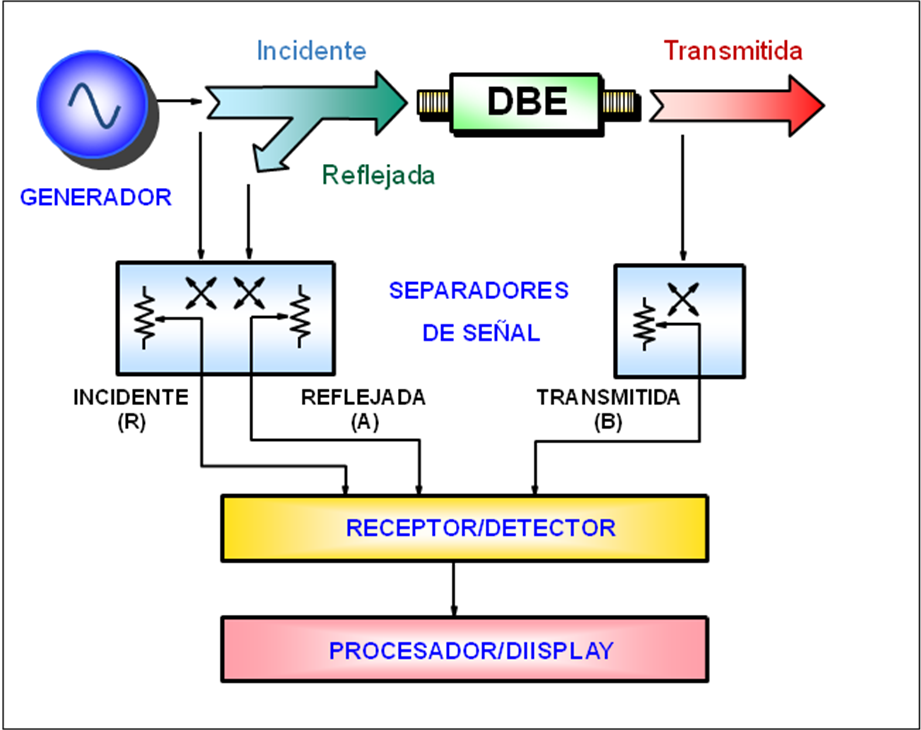
\includegraphics[width=\textwidth]{../img/analizador_redes.png}
    %    \caption{Bloques del amplificador}
    %   \label{}
\end{figure}

\subsubsection{Acoplador direccional}
Para dar comienzo al proceso de medición con un analizador de redes es fundamental separar
las señales incidente, reflejada y transmitida. En microondas es común utilizar acopladores
direccionales. Las propiedades más importantes para los acopladores direccionales son
disponer de un ancho de banda amplio, alta directividad y una buena impedancia de
adaptación en todos los puertos cuando los otros puertos están conectados a cargas
adaptadas terminadas en $Z_O$ .
En la figura siguiente se observa que el acoplador direccional tiene 4 puertos entrada, salida,
acoplado y aislado, la línea entre los puertos 1 y 2 se conocen como “línea principal".

\begin{figure}[H]
    \centering
    
\includegraphics[width=0.8\textwidth]{../img/acople_direccional.png}
    %    \caption{Bloques del amplificador}
    %   \label{}
\end{figure}

\begin{figure}[H]
    \centering
    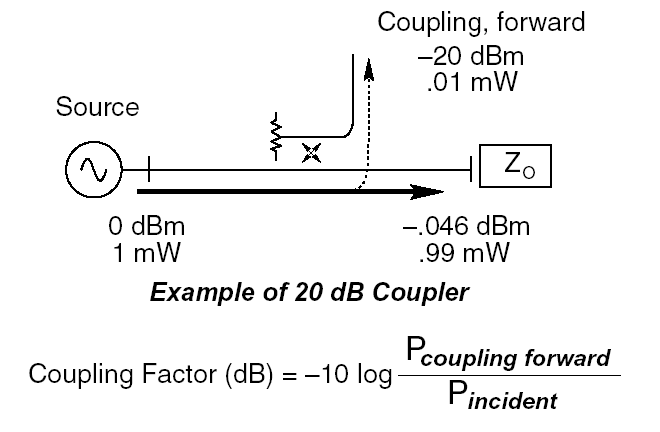
\includegraphics[width=0.8\textwidth]{../img/acople_direccional2.png}
    %    \caption{Bloques del amplificador}
    %   \label{}
\end{figure}

En un acoplador direccional ideal, las pérdidas de la línea principal desde el puerto 1 al puerto 2 (P1 – P2) debido a la potencia acoplada al puerto de salida son:
\begin{equation*}
loss = 10*\log*(1-\frac{P3}{P1})dB
\end{equation*}

Las pérdidas son una combinación de pérdidas de acoplamiento, pérdidas dieléctricas,
pérdidas del conductor y pérdidas por ROE.

\begin{figure}[H]
    \centering
    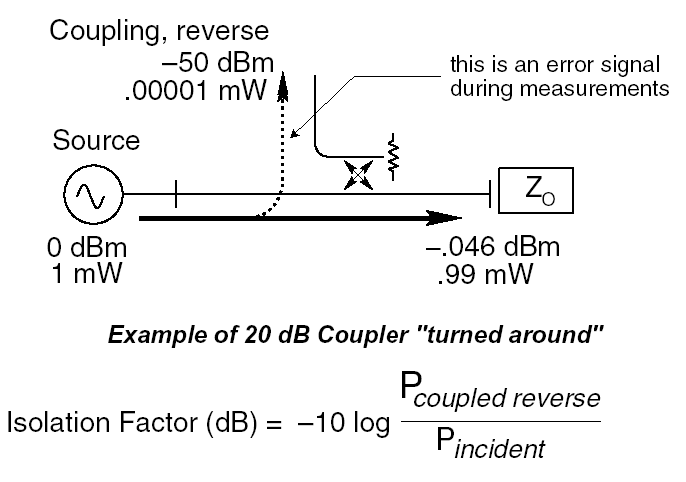
\includegraphics[width=0.8\textwidth]{../img/acople_direccional3.png}
    %    \caption{Bloques del amplificador}
    %   \label{}
\end{figure}

El aislamiento de un acoplador direccional puede ser definido como la diferencia en niveles de
señal, en dB, entre el puerto de entrada (P 1 ) y el puerto aislado (P 4 ) , estando los otros dos
puertos conectados a cargas adaptadas.

\begin{figure}[H]
    \centering
    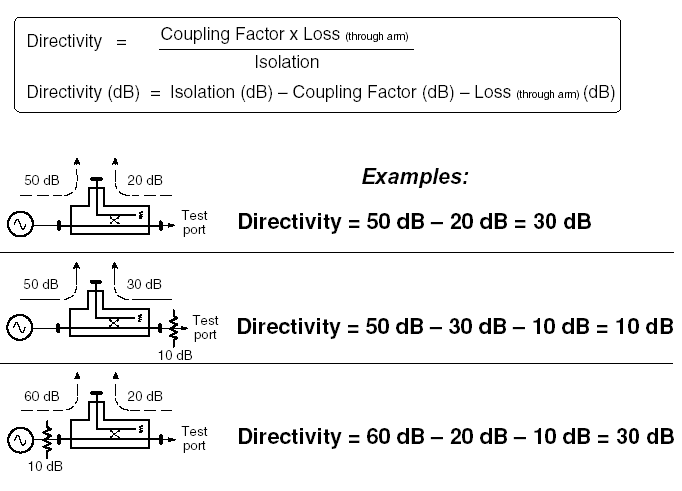
\includegraphics[width=0.8\textwidth]{../img/acople_direccional4.png}
    %    \caption{Bloques del amplificador}
    %   \label{}
\end{figure}

La directividad debería ser lo más alta posible, no es medible directamente, y es
calculada a partir de la diferencia entre las medidas de aislamiento, acoplamiento y
pérdidas:
Directividad($dB$) = $Aislamiento$ - $Acoplamiento$ - $Pérdidas$

\section{Analizador de Espectros}

\subsection{Diagrama en bloques}
\begin{figure}[H]
    \centering
    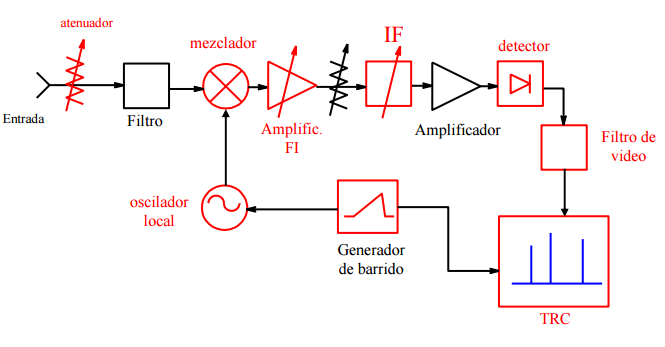
\includegraphics[width=0.8\textwidth]{../img/analizador_espectro.png}
    %    \caption{Bloques del amplificador}
    %   \label{}
\end{figure}

\subsection{Descripción de las etapas y controles principales}

\subsubsection{Atenuador de entrada:}

Es un atenuador ajustable por pasos de 10 dB entre 0 y 70 dB. Se encuentra entre el conector de
entrada y el preselector o bien la primera etapa mezcladora del analizador.
Puede funcionar en modo automático o manual.
En modo automatico el atenuador ajusta el nivel de la señal que entra en el primer mezclador para obtener un margen
dinámico máximo sin interferencias y una buena relación S/N.

El modo manual se utiliza para poder optimizar otros parámetros como sensibilidad o intermodulación.

\subsubsection{ Preselector:}
El preselector puede ser:
Un filtro pasabajos coincidente con la máxima frecuencia medible para los analizadores de
espectro de baja frecuencia o en el caso de analizadores de espectro de microondas, coincidente
con el primer rango de frecuencias donde el oscilador interno trabaja con su fundamental.
Un Filtro YIG Sintonizado (YTF) para los rangos superiores de frecuencia en los analizadores de
espectro de microondas. Este filtro solo permite que pase una determinada porción del espectro
moviéndose acorde a la frecuencia sintonizada del oscilador local (LO). Esto sirve para eliminar
el problema de múltiple batido.
La función del preselector es entonces eliminar toda frecuencia imagen, respuesta espuria y otras
que suelen aparecer para evitar falsas mediciones.

\subsubsection{Oscilador Local: LO}
Es el oscilador que genera la señal de heterodinación de las etapas mezcladoras. Pueden haber
dos, tres o más de estos dependiendo principalmente de la cantidad de mezcladores que haya. Se
suelen heterodinar sus fundamentales o sus armónicas según los rangos de frecuencia:
La ecuación de sintonía es la siguiente:
$ f_{in} = f_{LO} \pm f_{FI} $


\subsubsection{Diodo como detector de envolventes:}
\begin{figure}[H]
    \centering
    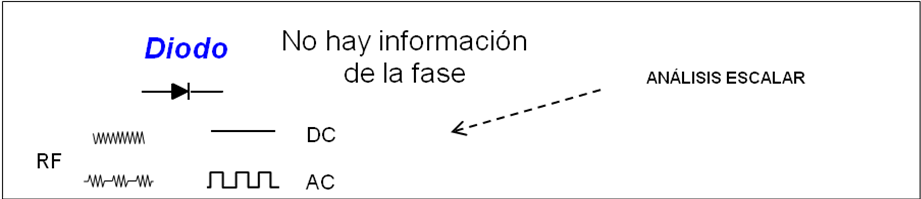
\includegraphics[width=0.8\textwidth]{../img/diodo2.png}
    %    \caption{Bloques del amplificador}
    %   \label{}
\end{figure}

Diodo detector. Es la solución más simple y económica en la que se
aprovecha la característica cuadrática propia del diodo para detectar la
potencia de la señal para cualquier frecuencia.

\begin{figure}[H]
    \centering
    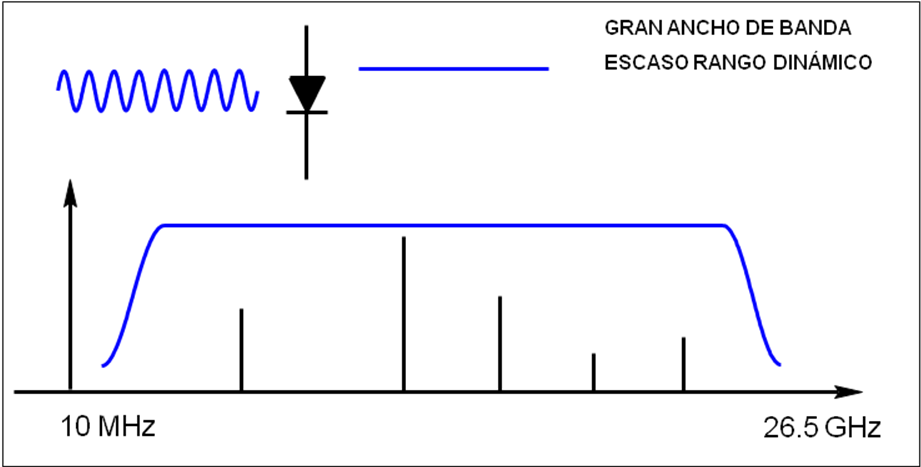
\includegraphics[width=0.8\textwidth]{../img/diodo.png}
    %    \caption{Bloques del amplificador}
    %   \label{}
\end{figure}


\subsubsection{Receptor sintonizado:}

Básicamente es un circuito superheterodino compuesto por un mezclador y un filtro pasabanda
sintonizado a una determinada frecuencia intermedia ( ó un amplificador de FI). Se trata, de un
receptor de banda estrecha cuya salida contiene la información de la señal de entrada
trasladada a la frecuencia intermedia.
\begin{figure}[H]
    \centering
    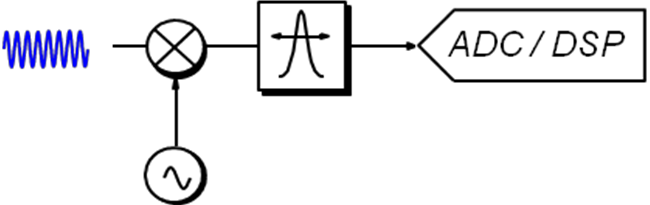
\includegraphics[width=0.8\textwidth]{../img/sintonizado.png}
    %    \caption{Bloques del amplificador}
    %   \label{}
\end{figure}
\begin{figure}[H]
    \centering
    
\includegraphics[width=0.8\textwidth]{../img/sintonizado2.png}
    %    \caption{Bloques del amplificador}
    %   \label{}
\end{figure}

\subsubsection{Control de Sintonía: Frecuencia Central}

Ajusta el LO para visualizar la señal a medir de tal forma que en el centro de la pantalla la
frecuencia sea: $f_{central}$ = $f_{LO}$ - $f_{FI}$
En el caso de medición a fullband posiciona la frecuencia central a $f_{MAX} / 2$ o en los antiguos
analizadores, posiciona una marca en frecuencia en la pantalla.

\subsubsection{Intervalo de frecuencia Span:}

Como el LO barre en forma lineal en frecuencia, el SPAN es el ancho de este barrido . Se lo
expresa en Hz/div de pantalla. En nuestro caso se extiende entre 1 kHz/div y 500 MHz/div.

\subsubsection{Barrido en toda la banda de frecuencia: Fullband sweep}

Es el barrido en todo el rango de frecuencias del analizador según las distintas bandas. En la
pantalla se puede observar todo el espectro de la señal siendo una función útil para identificar
distintas señales, ver la pureza espectral, etc. 

\subsubsection{ Barrido cero: Zero Span}
Es un modo de funcionamiento en el cual el barrido en frecuencia del oscilador local se ajusta a
cero. Esto permite efectuar medidas de nivel a frecuencias fijas y también poder representar una
señal en el dominio del tiempo (por ejemplo ver la señal modulante en AM, FM, pulso, etc.). 

\begin{figure}[H]
    \centering
    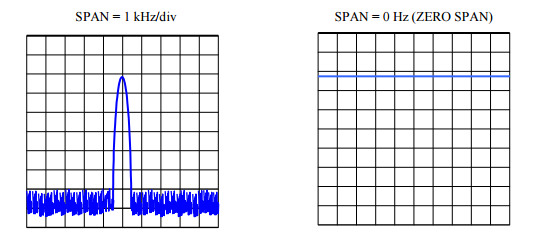
\includegraphics[width=0.8\textwidth]{../img/span.png}
    %    \caption{Bloques del amplificador}
    %   \label{}
\end{figure}

\subsubsection{Circuito de estabilización:}

Debido a las inestabilidades propias del oscilador y su FM residual, entre otras, por debajo de
cierto Span de barrido (100 kHz/div) actúa en forma automática el circuito de estabilización el
cual enclava al oscilador YTO a un oscilador de referencia de 1 MHz a cristal. Una vez
enclavado permite efectuar un ajuste fino en frecuencia.
Otra posibilidad podría ser dejar fijo al primer LO (coincidente con la frecuencia central en la
pantalla) y barrer el ultimo LO.

\subsubsection{Base de tiempo: Time Base}
Es la referencia en frecuencia que utiliza el sintetizador interno. Por lo tanto es la que determine
la estabilidad del analizador.

\subsubsection{ Salida de Calibración:}
Consta de una señal de frecuencia y amplitud determinadas con un cierta incertidumbre
(100 MHz / -10 dBm). Esto se utiliza para verificar el correcto funcionamiento del analizador. 

\subsubsection{Nivel de Referencia:}
Es el valor de referencia para todas las medidas de nivel. Se encuentra situado en el tope de la
pantalla. Las mediciones efectuadas con nivel de referencia poseen la máxima exactitud, ya que
desaparece el error de linealidad o error de subdivisión de escala.
El nivel de referencia depende de:
El valor del atenuador de entrada y la ganancia del amplificador de FI.

\subsubsection{Filtro de FI: Ancho de banda de resolución RBW}
Consta de una serie de filtros pasabanda seleccionables de diferentes ancho de banda
situados en la ultima FI.
En general están especificados para 3 dB del filtro de FI que efectúa la selección de la
señal. El ancho de banda de resolución define la selectividad de un analizador para señales
de idéntica amplitud. Es decir que no se puede medir dos componentes de la misma
amplitud separadas en frecuencia menos que el valor de RBW como se muestra en la
figura:

\begin{figure}[H]
    \centering
    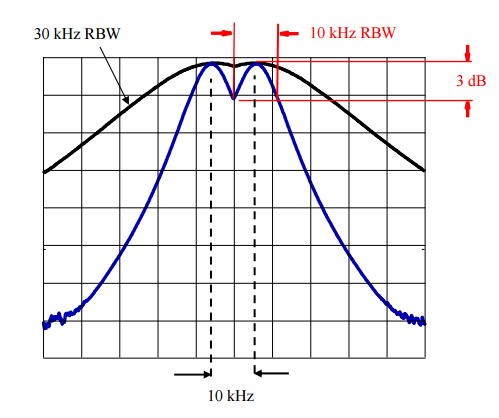
\includegraphics[width=0.8\textwidth]{../img/analizador_espectro2.png}
    %    \caption{Bloques del amplificador}
    %   \label{}
\end{figure}

\subsubsection{Ancho de banda de video: VBW}

Es el ancho de banda del filtro pasabajos que se encuentra después del detector.
A través de este se proporciona una constante de tiempo al análisis de nivel/amplitud, con lo cual
produce un filtrado (promedio) de las componentes de ruido de la señal medida. 

\subsubsection{Ruido}

El ruido generado en el analizador es aleatorio y tiene una amplitud constante para un
espectro de frecuencias muy amplio. Como el filtro de resolución esta ubicado después de
la primera etapa de ganancia, la potencia total de ruido que pasa a través este filtro, está
determinada por su ancho de banda, de modo que cuanto mas angosto es el filtro, menor
será el ruido que este deje pasar, como lo muestra la siguiente figura:

\begin{figure}[H]
    \centering
    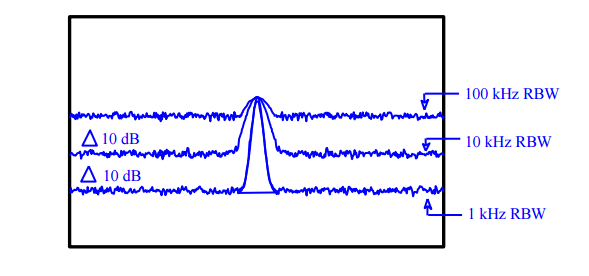
\includegraphics[width=0.8\textwidth]{../img/ruido.png}
    %    \caption{Bloques del amplificador}
    %   \label{}
\end{figure}

El nivel de ruido de fondo es función del log (RBW1 / RBW2), por lo tanto, si se
disminuye el RBW en un factor de 10 veces, el nivel de ruido mostrado disminuirá en 10
dB.
Entonces se logrará la mejor sensibilidad usando el mínimo RBW posible. 

\subsubsection{Ruido de Fase}

Debido a los efectos no lineales del oscilador, se produce la modulación de bandas laterales
de ruido, cuya potencia disminuye con la separación creciente de la portadora.
Se distingue entre ruido de amplitud (comportamiento estadístico de la estabilidad de
amplitud) y ruido de fase (comportamiento estadístico de la estabilidad de frecuencia/fase).

El ruido de fase es la magnitud principal:
Se define como la potencia absoluta de una banda lateral separada en $f_{off}$ de la
frecuencia de portadora, referida a la potencia de esta y con un ancho de banda
de prueba de 1 Hz. Su unidad es dBc/Hz.Como el ruido de fase se traslada a la FI,
constituye, conjuntamente con la selectividad, una indicación de la
resolución del analizador para señales de distinta amplitud y de frecuencias muy
próximas entre sí.
En la siguiente figura se observa como el ruido de fase enmascara a una componente
situada muy próximo a la componente fundamental. 

\begin{figure}[H]
    \centering
    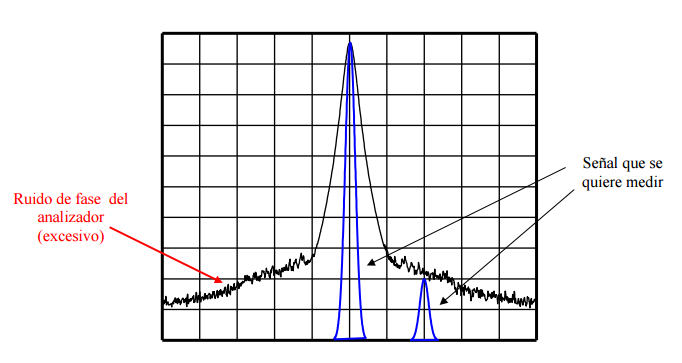
\includegraphics[width=0.8\textwidth]{../img/ruido_de_fase.png}
    %    \caption{Bloques del amplificador}
    %   \label{}
\end{figure}

\section{Parametros S}
Los parámetros de dispersión son los coeficientes de reflexión y transmisión entre la
onda incidente y la reflejada. Estos parámetros describen completamente el comportamiento
de un dispositivo bajo condiciones lineales en determinado rango de frecuencia. Cada
parámetro es caracterizado por magnitud, ganancias o pérdidas en decibeles y fase. A
pesar de ser aplicables a cualquier frecuencia, los parámetros S son usados principalmente
para redes que operan en radiofrecuencia (RF) y frecuencias de microondas. En general, para
redes prácticas, los parámetros S cambian con la frecuencia a la que se miden, razón por la
cual se debe especificar la frecuencia para cualquier medición de parámetros S, junto con la
impedancia característica o la impedancia del sistema.
En el contexto de los parámetros-S, dispersión se refiere a la forma en que las corrientes y
tensiones que se desplazan en una línea de transmisión son afectadas cuando se
encuentran con una discontinuidad debido a la introducción de una red en una línea de
transmisión. Esto equivale a la onda encontrándose con una impedancia diferente de la
impedancia característica de la línea.
La descripción de los parámetros es la siguiente:
\newline
$S_{11}$: Coeficiente de reflexión a la entrada o coeficiente de reflexión directa.
\newline
$S_{21}$: Coeficiente de transmisión directa o ganancia con la tensión directa.
\newline
$S_{22}$: Coeficiente de reflexión a la salida o coeficiente de reflexión inversa.
\newline
$S_{12}$: Coeficiente de transmisión o ganancia con la tensión inversa.
Para que esto sea valido las impedancias en el puerto de entrada y salida deben ser las
mismas.

La Figura 5a, muestra el esquema típico de un cuadripolo lineal, el cual puede estar
compuesto por elementos tanto activos como pasivos en su interior. La Figura 5b, muestra el
cuadripolo con los parámetros S.

\begin{figure}[H]
    \centering
    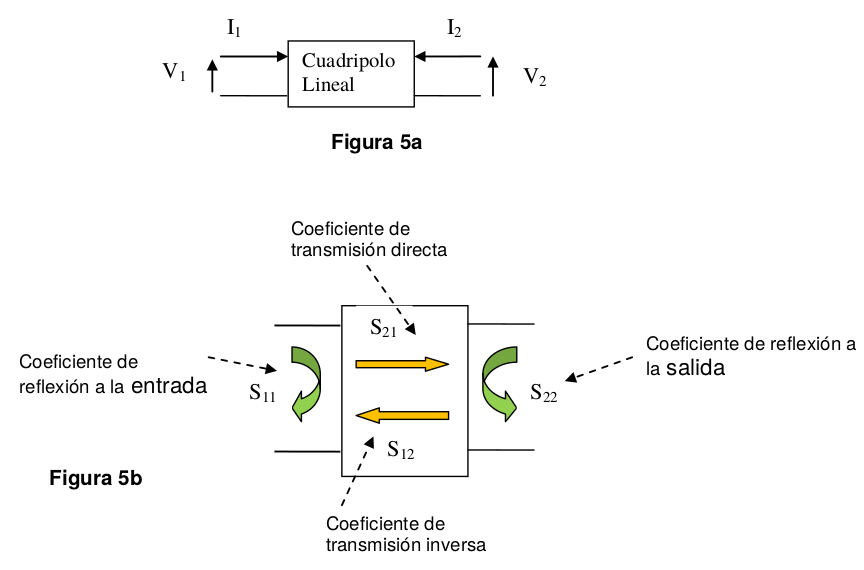
\includegraphics[width=0.8\textwidth]{../img/parametros_s.png}
    %   \caption{Bloques del amplificador}
    %   \label{}
\end{figure}

En la Figura siguiente se representa un cuadripolo con los parámetros S y el flujo de ondas
incidentes y reflejadas en cada uno de los puertos.

\begin{figure}[H]
    \centering
    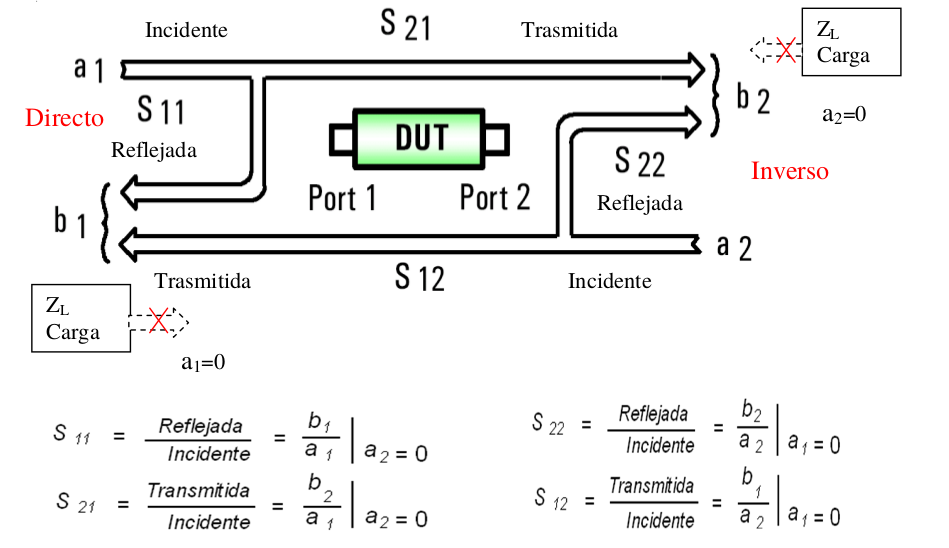
\includegraphics[width=0.8\textwidth]{../img/parametros_s2.png}
    %   \caption{Bloques del amplificador}
    %   \label{}
\end{figure}

Lo interesante de este esquema, es que se pueden determinar los parámetros S a partir de
mediciones de ondas incidentes y reflejadas en cada uno de los puertos para las condiciones
de $a_2$ = $0$ y $Z_L$ = $Z_0$; luego se procede a la inversa con $a_1$ = $0$ y $Z_1$ = $Z_L$ = $Z_0$.

\section{Carta Smith}
Cuando se miden los parámetros S, por cuestiones de aplicaciones en Investigación y
desarrollo de dispositivos o con fines industriales de producción, se debe considerar no
solamente la magnitud sino la fase involucrada con cada parámetro. Magnitud y fase de
dispositivos y redes describen con precisión el comportamiento con la frecuencia de RF
y microondas.
Las características en el dominio del tiempo necesitan de magnitud y fase para determinar las
correcciones vectoriales, como se indica en la siguiente figura.
\begin{figure}[H]
    \centering
    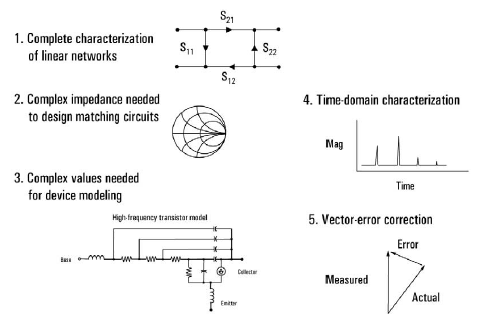
\includegraphics[width=0.8\textwidth]{../img/smith.png}
    %   \caption{Bloques del amplificador}
    %   \label{}
\end{figure}
Es clave, en líneas de transmisión la impedancia característica $Z_O$ ya que sirve para determinar
la relación entre corriente y tension de ondas en desplazamiento (traveling). Es una función de
la dimensión de la línea de transmisión y de la constante dieléctrica del material no
conductor de la línea. Para sistemas de RF, $Z_O$ es de 50 o 75 $\Omega$. Para potencia baja, como
cable de TV, la línea de transmisión coaxial está optimizada para bajas pérdidas y es de 75 $\Omega$,
con aire como dieléctrico. Para RF y microondas con aplicaciones de potencia elevada se
utiliza línea de transmisión coaxial con $50\Omega$, con una relación entre máxima potencia y
mínima pérdida.
Para máxima transferencia de energía a través de una línea de transmisión desde la fuente a la
carga deben tener la misma impedancia $Z_O$.
Cuando la impedancia de la fuente no es resistiva pura, la máxima transferencia de
energía ocurre cuando la impedancia de la carga o de salida es igual al complejo
conjugado de la impedancia de la fuente.
En este último caso se trabaja con la parte inversa de la señal y la parte imaginaria de la
impedancia. Ej: Si $RS = 0.6 + j0.3 (\Omega)$, el complejo conjugado es $RS*= 0.6-j0.3 (\Omega)$. La fuente de
señal se ajusta al complejo conjugado de la impedancia de carga o de salida.
Por lo tanto cuando se está en la etapa de diseño de un dispositivo, el Amplificador de RF
cubre el rango de frecuencia de la impedancia de carga, que es la impedancia de la antena.
Esta es una de las características de diseño en amplificadores de RF para máxima
transferencia de energía. Es importante considerar los parámetros de reflexión y de
transmisión, así como el contenido de
la figura siguiente.
Haciendo una ampliación de la Carta de Smith de la anterior se obtiene:
\begin{figure}[H]
    \centering
    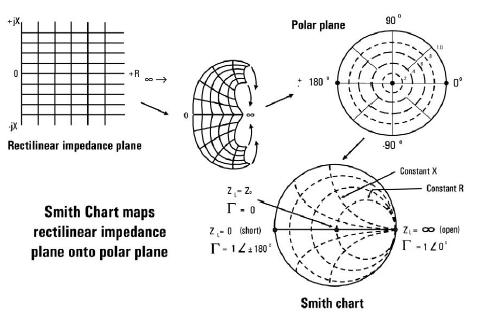
\includegraphics[width=0.8\textwidth]{../img/smith2.png}
    %    \caption{Bloques del amplificador}
    %   \label{}
\end{figure}

Como el coeficiente de reflexión $\Phi$, también denominado \textbf{r} , es una cantidad compleja, con magnitud y fase, para definirla correctamente debe tener ambas partes. La carta de Smith
método gráfico para tratar el tema de los parámetros S. Como la impedancia es un
En general, la Carta de Smith está normalizada para $Z_O$, de tal manera que los valores de
impedancia están divididos por $Z_O$ , con lo cual se hace independiente de las impedancias
del sistema bajo análisis.
En la computadora se visualiza el gráfico de Smith y el coeficiente de reflexión, mediante un
display polar.
Los valores de la impedancia se derivan por multiplicación del valor indicado para $Z_O$. En un
sistema de $\SI{50}\ohm$, un valor normalizado de $0.3 - j0.15 \Omega$  deriva en $15 - j7.5 \Omega$; en un
sistema de $\SI{75}\ohm$  es $22.5 - j 11.25 \Omega$.

\section{Mixer}
Un Mixer o Mezclador, es un circuito en los que se mezclan dos señales para producir frecuencias suma o resta deseadas. El receptor superheterodino inventado por Armstrong fue el primero en usar una etapa mezcladora (que llamó el "primer detector") para convertir la señal incidente de RF en una frecuencia intermedia más baja.
Cualquier dispositivo no lineal puede servir como mezclador: la alinealidad se requiere para producir frecuencias
no presentes a la entrada. De este modo, los mezcladores pueden usar diodos, BJTs, FETs o aún reactores saturables.
Las elecciones de diseño giran sobre consideraciones de ganancia (o pérdida), cifra de ruido, estabilidad, 
rango dinámico y la posible generación de frecuencias indeseables que produzcan intermodulación y distorsión.

Un mezclador de terminación única muy sencillo, se puede construir como se ilustra en la figura 7.3, como un
diodo en serie con las entradas de RF y de oscilador local (LO), una fuente de polarización y un circuito sintonizado
 a la frecuencia de FI deseada.
Sin embargo, un mezclador como el mencionado tiene bastantes desventajas. Posee a) una cifra de ruido relativamente alta;
 b) pérdida por conversión es decir, la salida de potencia de señal FI es menor que la entrada de potencia de señal (RF);
 c) no linealidades de orden superior, dada la característica brusca de corte del diodo; d) ningún
aislamiento entre el LO y las entradas de RF, incrementando así la posibilidad de que la señal del LO puede inyectarse
 a la antena receptora y e) una corriente de salida relativamente intensa en la frecuencia del LO, tiende a sobrecargar la etapa de entrada de FI.
En la figura 7.4 se muestran tres mezcladores de terminación única que usan FETs. En la 7.4a, la señal del LO
se inyecta directamente a la compuerta del FET, junto con la señal de RF. Comparando con el mezclador a diodo,
tiene ganancia de conversión y una cifra de ruido más baja; las no linealidades de orden superior se reducen al mínimo 
mediante la característica de transferencia de ley cuadrática, aproximadamente. Se puede sustituir el BJT por
un JFET para obtener más ganancia, pero la distorsión de tercer orden se incrementa también marcadamente.

\begin{figure}[H]
    \centering
    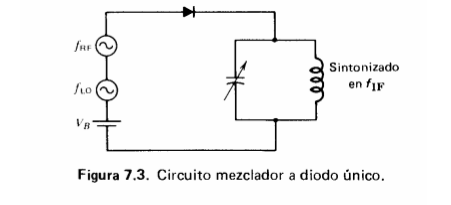
\includegraphics[width=0.8\textwidth]{../img/mezclador2.png}
    %    \caption{Bloques del amplificador}
    %   \label{}
\end{figure}

\begin{figure}[H]
    \centering
    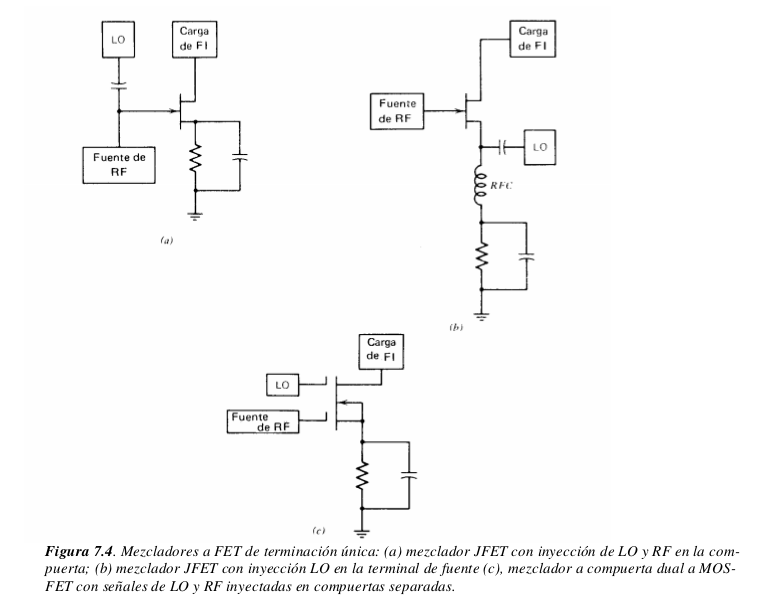
\includegraphics[width=0.8\textwidth]{../img/mezclador3.png}
    %    \caption{Bloques del amplificador}
    %   \label{}
\end{figure}


\subsection{Funcionamiento del mezclador}

Los siguientes términos se usan para describir el funcionamiento del mezclador:
\newline
\textbf{Ganancia (o pérdida) de conversión} es la razón de la potencia de señal de salida (FI) a la de entrada
(RF)
\newline
\textbf{Cifra de ruido es la SNR} (relación señal-a-ruido) en el puerto de entrada (RF) dividida entre el SNR en
el puerto de salida (FI).
\newline
El \textbf{aislamiento} representa la cantidad de fuga o paso de alimentación entre los puertos del mezclador. Sea $f_{RF}$ la frecuencia en el puerto de RF, $f_{LO}$ la del oscilador local y $f_{IF}$ la de FI. Entonces el aislamiento
 en el puerto RF en $f_{LO}$ es la cantidad en que la señal de nivel de excitación se atenúa cuando se
mide en el puerto de RF. El aislamiento en el puerto FI en $f_{LO}$ es la cantidad en que la señal de nivel
de excitación se atenúa cuando se mide en el puerto FI.
\newline
La \textbf{compresión de conversión} se refiere al nivel de potencia de entrada RF arriba del cual la curva de
potencia de salida FI vs potencia de entrada RF se desvía de la linealidad. Arriba de este nivel, un aumento
 adicional en el nivel de entrada RF no se traduce en un aumento proporcional en el nivel de salida. 
Cuantitativamente, la compresión de conversión es la reducción del nivel de salida en dB abajo de la
característica lineal. Usualmente, el nivel de entrada en el que la compresión es de 1 o 3 dB se da en las
especificaciones del mezclador (ver figura 7.5)
El rango dinámico es el rango de amplitud dentro del cual el mezclador puede trabajar sin degradación
en la operación. Depende del punto de compresión de conversión y de la cifra de ruido del mezclador.

\begin{figure}[H]
    \centering
    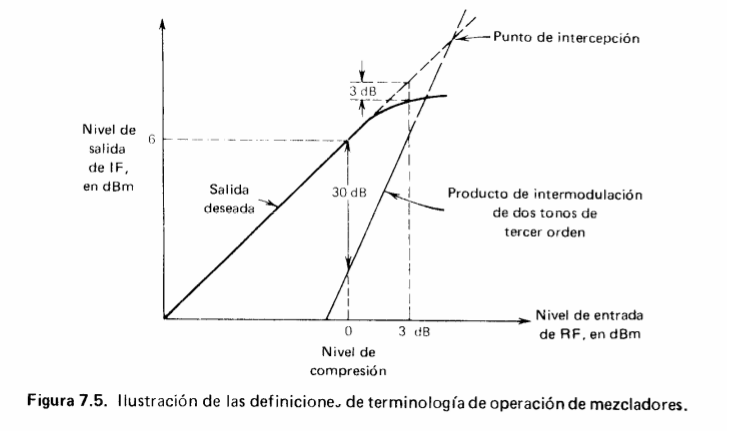
\includegraphics[width=0.8\textwidth]{../img/mezclador.png}
    %    \caption{Bloques del amplificador}
    %   \label{}
\end{figure}


\section{AM-FM}
\subsection{Modulación de Amplitud}
Modulación de amplitud (AM) es el proceso de cambiar la amplitud de una portadora de frecuencia relativamente
alta de acuerdo con la amplitud de la señal modulante (información) Las frecuencias que son lo suficientemente altas
para radiarse de manera eficiente por una antena y propagarse por el espacio libre se llaman comúnmente radiofrecuencias o simplemente RF. 
Con la modulación de amplitud, la información se imprime sobre la portadora en la forma de cambios de amplitud. 
La modulación de amplitud es una forma de modulación relativamente barata y de baja calidad de transmisión,
 que se utiliza en la radiodifusión de señales de audio y vídeo.
Un modulador de AM es un aparato no lineal con dos señales de entrada: a)una señal portadora de amplitud constante 
y de frecuencia única y b)la señal de información. La información “actúa sobre” o “modula” la portadora y puede
ser una forma de onda de frecuencia simple o compleja compuesta de muchas frecuencias que fueron originadas de una o
más fuentes. Debido a que la información actúa sobre la portadora, se le llama señal modulante. La resultante se llama
onda modulada o señal modulada.

\subsubsection{Espectro de frecuencia de AM y ancho de banda}
Un modulador AM es un dispositivo no lineal . Por lo tanto, ocurre una mezcla no lineal (producto) y la envolvente de salida es una onda compleja compuesta por una tensión de c.c., la frecuencia portadora y las frecuencias de suma ( $f_c$ + $f_m$ ) y diferencia ($f_c$ - $f_m$ ) (es decir, los productos cruzados).
 La suma y la diferencia de frecuencias son desplazadas de la frecuencia portadora por una cantidad igual a la frecuencia de la señal modulante.
Por lo tanto, una envolvente de AM contiene componentes en frecuencia espaciados por “f m ” Hz en cualquiera de los
lados de la portadora. Sin embargo, debe observarse que la onda modulada no contiene una componente de frecuencia
que sea igual a la frecuencia de la señal modulante. El efecto de la modulación es trasladar la señal de modulante en el
dominio de la frecuencia para reflejarse simétricamente alrededor la frecuencia de la portadora.
La figura 3-2 muestra el espectro de frecuencia para una onda de AM.
El espectro de AM abarca desde ($f_c$ - $f_{max}$) a ($f_c$ + $f_{max}$ ) en donde $f_c$ es la frecuencia de la portadora y $f_m$ (max) es la frecuencia de la señal modulante más alta. 
La banda de frecuencias entre $f_c$ - $f_m$ (max) y $f_c$ se llama banda lateral inferior (LSB) y cualquier frecuencia dentro de esta banda
se llama frecuencia lateral inferior (LSF). La banda de frecuencias entre $f_c$ y $f_c$ + $f_m$ (max) se llama banda lateral superior (USB) 
y cualquier frecuencia dentro de esta banda se llama frecuencia lateral superior (USF). 
Por lo tanto, el ancho de banda (B ó BW) de una onda AM DSBFC es igual a la diferencia entre la frecuencia lateral superior más alta
 y la frecuencia lateral inferior más baja o sea dos veces la frecuencia de la señal modulante más alta (es decir, B = $2f_m$)
Para la propagación de una onda radio, la portadora y todas las frecuencias dentro de las bandas laterales superiores e
inferiores debe ser lo suficientemente altas para propagarse por la atmósfera de la Tierra (incluida la ionosfera)
En la figura 3.4.bis(a) se ilustran las representaciones en el dominio de la frecuencia para la modulación de amplitud,
y en la figura 3.4.bis(b) se muestra la suma lineal de las dos señales. La señal de AM no tiene componente en la frecuencia
moduladora: toda la información se transmite a frecuencias cercanas a la de la portadora.
En contraposición, la suma lineal no logró nada: en el bosquejo del dominio de frecuencia se observa que las señales
de la información y la portadora están separadas, cada una a su frecuencia original.

\begin{figure}[H]
    \centering
    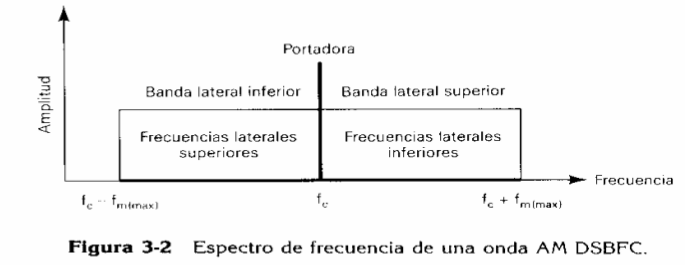
\includegraphics[width=0.8\textwidth]{../img/am.png}
\end{figure}

\begin{figure}[H]
    \centering
    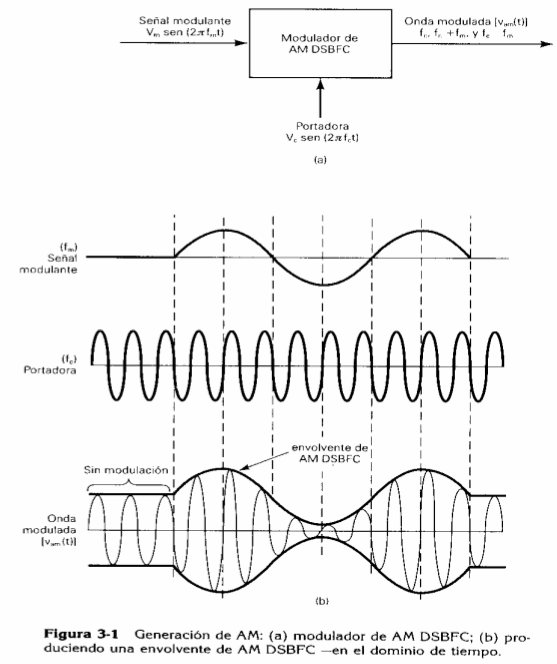
\includegraphics[width=0.8\textwidth]{../img/am2.png}
\end{figure}

\begin{figure}[H]
    \centering
    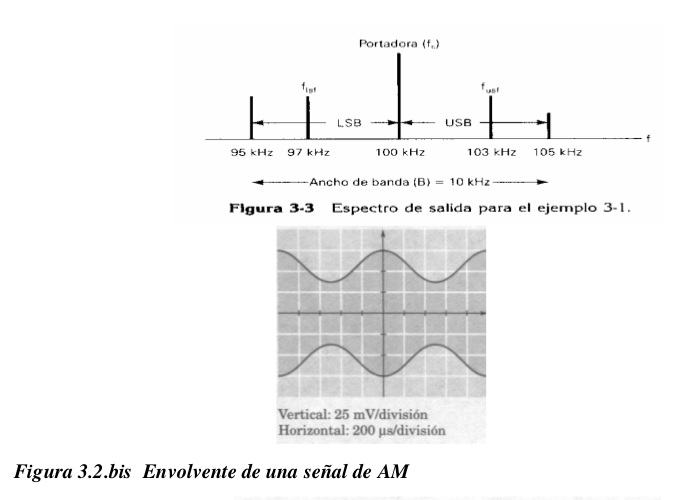
\includegraphics[width=0.8\textwidth]{../img/am3.png}
\end{figure}

\begin{figure}[H]
    \centering
    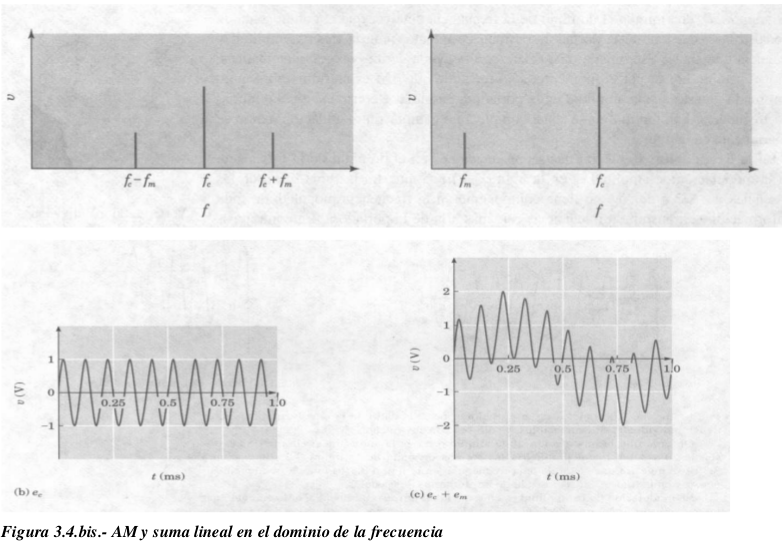
\includegraphics[width=0.8\textwidth]{../img/am4.png}
\end{figure}

\subsection{Indice M}

Coefeciente de modulación es un término utilizado para describir la cantidad de cambio de amplitud (modulación)
 presente en una forma de una onda de AM. El porcentaje de modulación es simplemente el coeficiente de modulación establecido como un porcentaje.
 Más específico, el porcentaje de modulación proporciona el cambio de porcentaje en la amplitud de la onda de salida cuando está actuando sobre la portadora por una señal modulante. Matemáticamente, el coeficiente de modulación es:

\begin{equation*}
m=\frac{E_m}{E_c}
\end{equation*}

en donde
\newline
$m$ = coeficiente de modulación (sin unidad)
\newline
$E_m$ = cambio pico en la amplitud de tensión de la forma de onda de salida (volts)
\newline
$E_c$ = amplitud pico de tensión de la portadora no modulada (volts)
La ecuación anterior puede rearreglarse para resolver a $E_m$ y $E_c$ como
\newline
$E_m$ = $m*E_c$ 
\newline
$E_c$ = $E_m$/$m$ 
\newline
y el porcentaje de modulación (M) es:
\newline 
$M$ = $E_m$/$E_c$ x 100

Las relaciones entre $m$, $E_m$ y $E_c$ se muestra en la figura 3-5.
Si la señal modulante es una onda seno pura de frecuencia simple y el proceso de modulación es simétrico (es decir, las excursiones positivas y negativas de la amplitud de la envolvente son iguales), el porcentaje de modulación puede derivarse de la siguiente manera (refiérase a la figura 3-5 para la siguiente derivación):
\newline
$E_m = \frac{1}{2} (V_{max} - V_{min} )$
\newline
$E_c = \frac{1}{2} (V_{max} + V_{min} )$
\newline
\newline
Por lo tanto:
\begin{figure}[H]
    \centering
    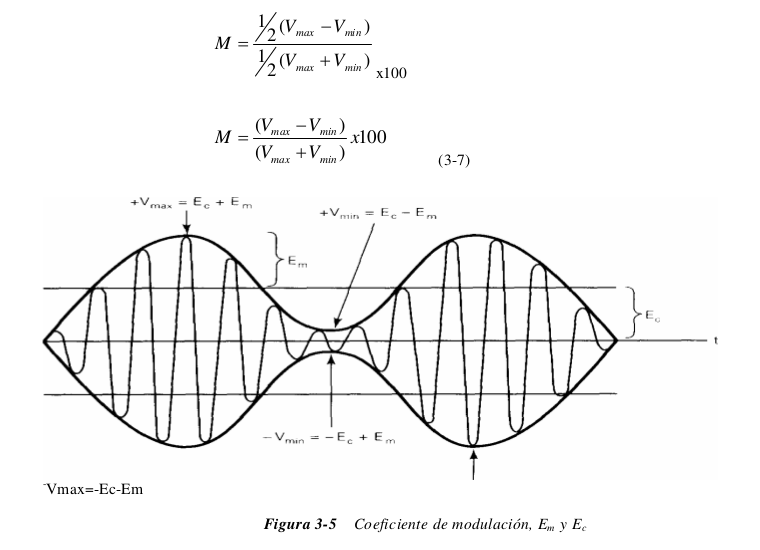
\includegraphics[width=0.8\textwidth]{../img/m.png}
\end{figure}

\section{Impedancimetro}


\section{Zin|z}
\begin{equation*}
Z_{in}=Z_0*\frac{Z_L+j*Z_0*\tan(\beta L)}{Z_0+j*Z_L*\tan(\beta L)}
\end{equation*}
\begin{equation*}
\beta=\frac{2\pi}{\lambda}
\end{equation*}
\section{Reflectometria}

El reflectómetro, básicamente utiliza una técnica de medición del coeficiente de reflexión y
de relación de onda estacionaria (ROE) en líneas de transmisión, obteniendo información
sobre distintos parámetros que permiten determinar el comportamiento de la misma ante
determinadas situaciones de cortocircuito, circuito abierto, atenuación, pérdidas, etc. En
principio mide: la onda de tension incidente y la onda reflejada; el tiempo que tarda el pulso
o un escalón en ir desde la entrada a la carga y volver al punto de entrada, dando el
coeficiente de reflexión $r$ de la carga y la ROE, en valor absoluto sin información sobre la
fase en los instrumentos más económicos. Además da la distancia a la que se encuentra
una discontinuidad a partir del tiempo que demora una señal en ir y volver desde la
entrada a la salida, y de la velocidad de propagación según cada tipo de cable utilizado en
una determinada red. Hay diferentes tipos de reflectómetros, desde un osciloscopio de
muestro con muy elevado tiempo de respuesta y amplio ancho de banda del orden de los
GHZ a instrumentos portátiles para detectar fallas en cables.

 En general podemos pensar en una onda que viaja hacia la carga y que se ve parcialmente “reflejada” en ella. 
Se observa que $r_L$ = $0$ si $Z_L$ = $Z_0$. En este caso no existe onda regresiva (no existe reflexión). La carga está adaptada a la línea, y esto ocurre cuando la impedancia de carga es igual a la impedancia característica de la línea. 
En el caso de una linea abierta con $Z_L$ infinito, el coeficiente de reflexión es 1, por lo que la onda se refleja completamente.
En una linea cortocircuitada la onda se refleja completamente tambien pero con un cambio de fase.

\begin{figure}[H]
    \centering
    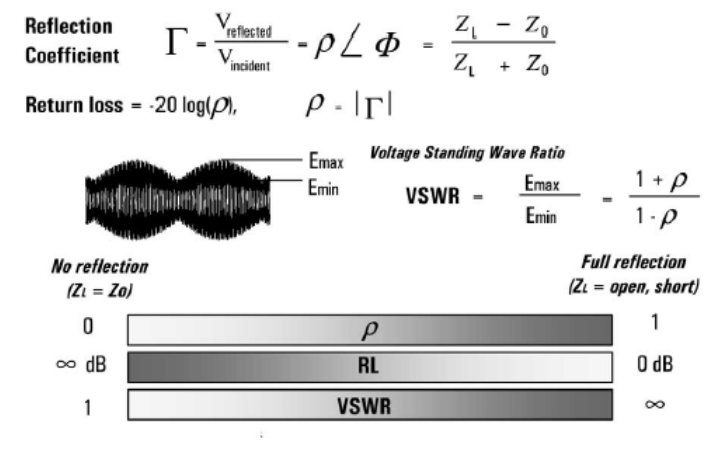
\includegraphics[width=0.8\textwidth]{../img/reflectometria.png}
    %    \caption{Bloques del amplificador}
    %   \label{}
\end{figure}

\subsection{Mediciones con TDR}

La Reflectometría en el Dominio del Tiempo (TDR), básicamente se comporta como un
radar de lazo cerrado, y consiste en un Generador de Función escalón que se conecta
por intermedio de un terminal $T_e$ (Acoplador Direccional) al
elemento que se quiere medir y a un osciloscopio para realizar la medición en dicho
punto.
En comparación con otras técnicas de medición, la reflectometría en el dominio del tiempo
proporciona un aspecto más directo para analizar las características de los DUT. Las
ondas incidentes y reflejadas de tension son controladas o monitoreadas, por el
osciloscopio en un punto determinado de la línea.
Esta técnica de eco, como se observa en la Figura 4, revela la impedancia característica
de la línea, muestra tanto la posición y la naturaleza (resistiva, inductiva o capacitiva) de
cada discontinuidad dada por la diferencia de materiales a lo largo de la línea. El TDR
también muestra si las pérdidas en un sistema de transmisión son las pérdidas de
elementos en serie o las pérdidas de elementos en derivación. Toda esta información
está disponible inmediatamente en la pantalla del osciloscopio.
La onda reflejada se identifica fácilmente ya que se separa en el tiempo de la onda incidente.
Este tiempo es importante para determinar la longitud de la red de transporte desde el punto de control o monitoreo. La distancia a la
que se encuentra la carga es D.
\begin{figure}[H]
    \centering
    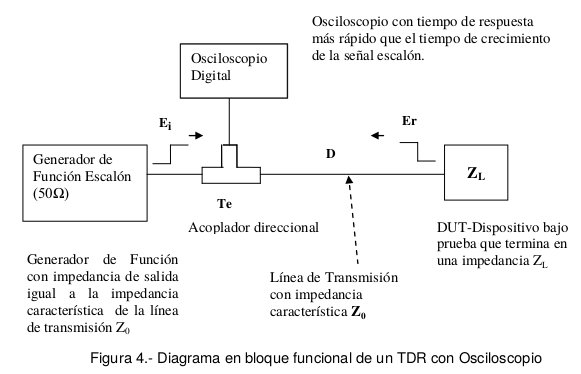
\includegraphics[width=0.8\textwidth]{../img/tdr.png}
    %    \caption{Bloques del amplificador}
    %   \label{}
\end{figure}
Se denomina impedancia característica, $Z_0$ , de una línea de transmisión a la relación existente entre la
diferencia de potencial aplicada y la corriente absorbida por la línea en el caso hipotético de que esta
tenga una longitud infinita, o cuando aún siendo finita no existen reflexiones. Para que no exista
reflexión en una línea de longitud finita, la misma impedancia que se presenta en su entrada
está en su salida, si esta última se termina en una impedancia igual a la impedancia
característica. Cuando está terminada en esa impedancia, toda la energía enviada por la línea
es absorbida por la carga y no hay reflexión.

La ddp escalón del generador , $E_i$ , se propaga a lo largo de la línea hasta llegar a la carga $Z_L$ , vía el acoplador direccional $T_ e$ que conecta las tres partes involucradas en la experiencia, el Generador , el Osciloscopio y la Línea de transmisión, y por ésta al
dispositivo que representa la Impedancia $Z_L$ o que termina en dicha impedancia.
Según como se comporte la carga se tendrán diferentes situaciones. Si la carga no produce reflexión, el coeficiente de reflexión es cero, $r$=$0$. Si la carga real produce reflexión, $r\neq0$  habrá un escalón reflejado $E_r$ y en el osciloscopio se observará lo que se
muestra en la Figura 4 y Figura 5.

\begin{figure}[H]
    \centering
    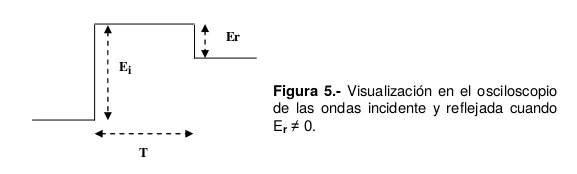
\includegraphics[width=0.8\textwidth]{../img/tdr2.png}
    %    \caption{Bloques del amplificador}
    %   \label{}
\end{figure}

El tiempo $T$, es el tiempo que tarda el frente del escalón $E_i$ en ir hacia la carga y en volver
como un escalón reflejado $E_r$ al punto $T_e$ de origen. Es fácilmente medido en el
Osciloscopio y es fundamental para determinar la distancia a la que se encuentra la carga
o alguna discontinuidad.
De la información presentada en el osciloscopio es posible determinar el coeficiente de
reflexión, $E_i$ / $E_r$ , y en consecuencia la relación de onda estacionaria ROE, el osciloscopio
digital tiene un firmware incorporado que permite presentar estos datos en forma
inmediata.
Si se conoce la velocidad de propagación $V_p$ , se puede convertir la información del
tiempo $T$ que proporciona el osciloscopio en distancia medida a partir del origen $T_e$ ,
obteniendo la distancia a la que se encuentra la carga $Z_L$.

\end{document}
